\documentclass{beamer}

\usepackage{tikz}
\usepackage{amsfonts}
\usepackage{amsmath}
\usepackage{mathabx}
\usepackage{amsthm}
\usepackage{graphicx}
\newtheorem{mydef}{Definition}

\usepackage[citestyle=alphabetic,bibstyle=numeric,hyperref,backend=biber]{biblatex}
\addbibresource{backprop.bib}
\bibhang1em

\title{Backpropagation}
\author{Leander Kurscheidt}
\institute{Hack \& S{\"o}hne}
\date{2018}
     

\begin{document}
 
\frame{\titlepage}
 
\begin{frame}
\frametitle{Backpropagation}
\begin{itemize}
    \item We've got the forward propagation, but how to train the neural network?
    \item many approaches, but Backward-Propagation is enabling the whole Deep-Learning Hype
\end{itemize}
for BP to work, \textbf{everything} needs to be differentiable!!!!
\end{frame}

\begin{frame}{Intuition: Learning as an Optimization-Problem}
in theory, it's easy!
\vfill
\begin{enumerate}
    \item assign every instance of neural network a score through a differentiable function (error function), e.g. derivation from target
    \item optimize the score
\end{enumerate}
\end{frame}

\begin{frame}{Intuition: Learning as an Optimization-Problem}
\begin{figure}
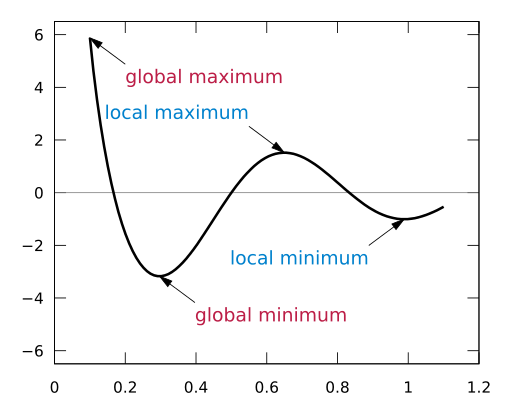
\includegraphics[scale=0.5]{../assets/512px-Extrema_example_original.png}
\caption{\cite{extremaMinima}}
\end{figure}
\end{frame}

\begin{frame}{Intuition: Learning as an Optimization-Problem}
    common vocabulary:
    \vfill
    \begin{enumerate}
        \item a \textbf{Loss-Function} $L$ is something I want to minimize
        \item an \textbf{Error-Function} $E : Output_{NN} \bigtimes Target \rightarrow \mathbb{R} $ \\
        $\Rightarrow$ in our context: Loss-Function = Error-Function
    \end{enumerate}
\end{frame}

\begin{frame}{Intuition: Learning as an Optimization-Problem}
    \begin{figure}
    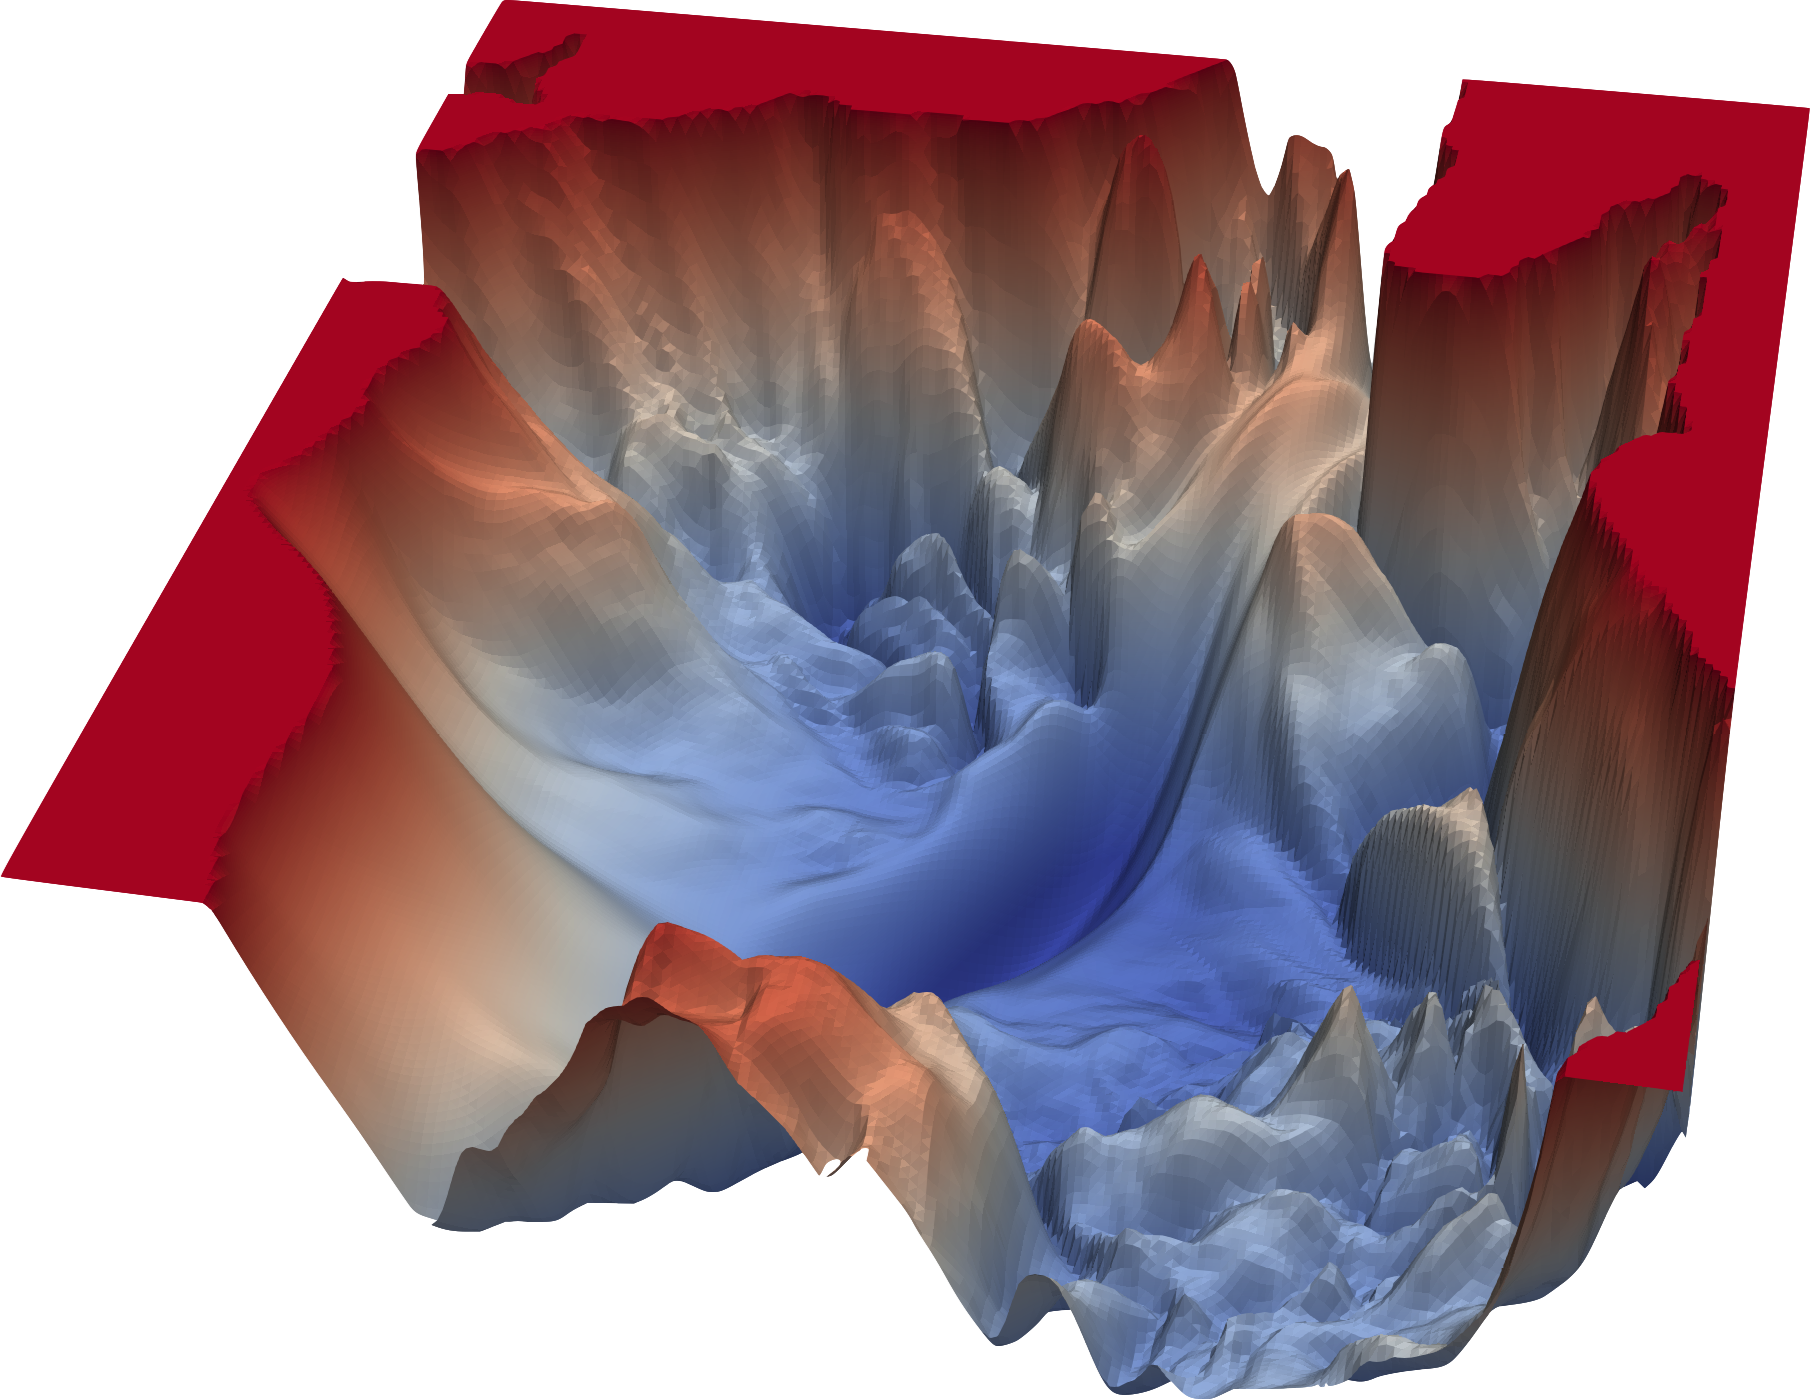
\includegraphics[width=\textwidth]{../assets/noshort.png}
    \caption{\cite{DBLP:journals/corr/abs-1712-09913}}
    \end{figure}
\end{frame}

\begin{frame}{The BP-Algorithm}
    \vfill
    \centering
    \begin{beamercolorbox}[sep=8pt,center,shadow=true,rounded=true]{title}
      \usebeamerfont{title}essentially: nothing more than the chain rule!
    \end{beamercolorbox}
    \vfill
\end{frame}

\begin{frame}{A naive formulation}
    $w_{ijz}$ is the weight $z$ of neuron $j$ in layer $z$\\
    Gradients of our Error Function: $\nabla E = \{\frac{\partial E}{\partial w_{1}}, \frac{\partial E}{\partial w_{2}}, ..., \frac{\partial E}{\partial w_{l}}\}$
    \vfill
    \pause\begin{mydef}
        update weight: $\Delta w_{ij} = - \lambda \cdot \frac{\partial E}{\partial w_{ij}}$, where $\lambda$ is the learning rate ("step size")
    \end{mydef}
\end{frame}

\begin{frame}{This is expensive!}
    \begin{figure}
        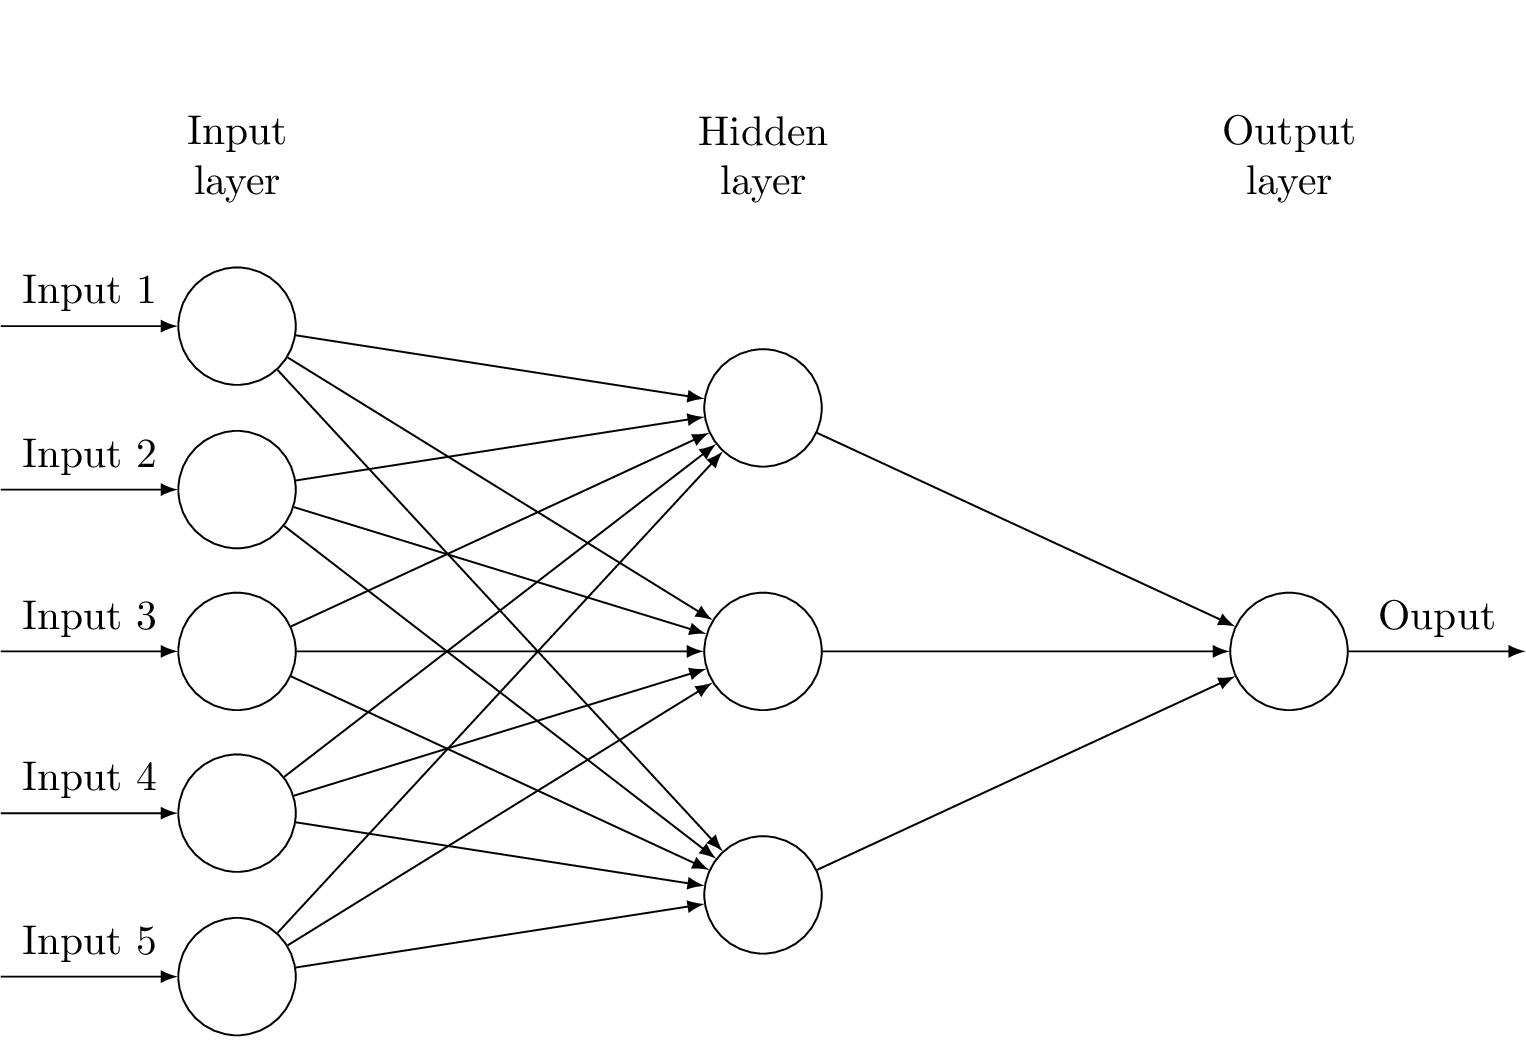
\includegraphics[width=0.8\textwidth]{../assets/mlp_model.png}
    \end{figure}
    \begin{itemize}
        \pause \item $5\cdot3+5+3+1=24$ weights!
        \pause \item often hundreds of thousands of weights in real scenarios!
        \pause \item and this is \textbf{one} update
    \end{itemize}
\end{frame}

\begin{frame}{Recap: Generalization of the Chain-Rule}
    single variable: $[f \circ g (x)]'= (f' \circ g)(x) \cdot g'(x)$\\
    different notation: for $y = f(t)$, $t = g(x)$: $\frac{d y}{d x} = \frac{d y}{d t}\frac{d t}{d x}$
    \vfill
    generalized to multivar.:\\ For $y = f(m_1,m_2)$,$m_1 = g(x_1,x_2)$ and $m_2 = h(x_1, x_2)$ :\\ $\frac{\partial y}{\partial x_1} = \frac{\partial y}{\partial m_1} \frac{\partial m_1}{\partial x_1} + \frac{\partial y}{\partial m_2} \frac{\partial m_2}{\partial x_1}$
\end{frame}

\begin{frame}{Chain rule to the rescue!}
    $w_{ij}$ is a weight $i$ of layer $j$
    \vfill
    \begin{align*}
        \Delta w_{ij} & = - \lambda \cdot \frac{\partial E}{\partial w_{ij}} \\
         \onslide<2-> {& = - \lambda \cdot \sum_{n = 0}^{l_{j+1}} \frac{\partial E}{\partial w_{n (j+1)}}\frac{\partial w_{n (j+1)}}{\partial w_{ij}} \\ }
         \onslide<3-> {& = - \lambda \cdot \sum_{n_1 = 0}^{l_{j+1}} \textcolor{blue}{(\sum_{n_2 = 0}^{l_{j+2}} \frac{\partial E}{\partial w_{n_2 (j+2)}}\frac{\partial w_{n_2 (j+2)}}{\partial w_{n_1 (j+1)}})} \frac{\partial w_{n_1 (j+1)}}{\partial w_{ij}} }
    \end{align*}
\end{frame}

\begin{frame}{Chain rule to the rescue!}
    \begin{figure}
        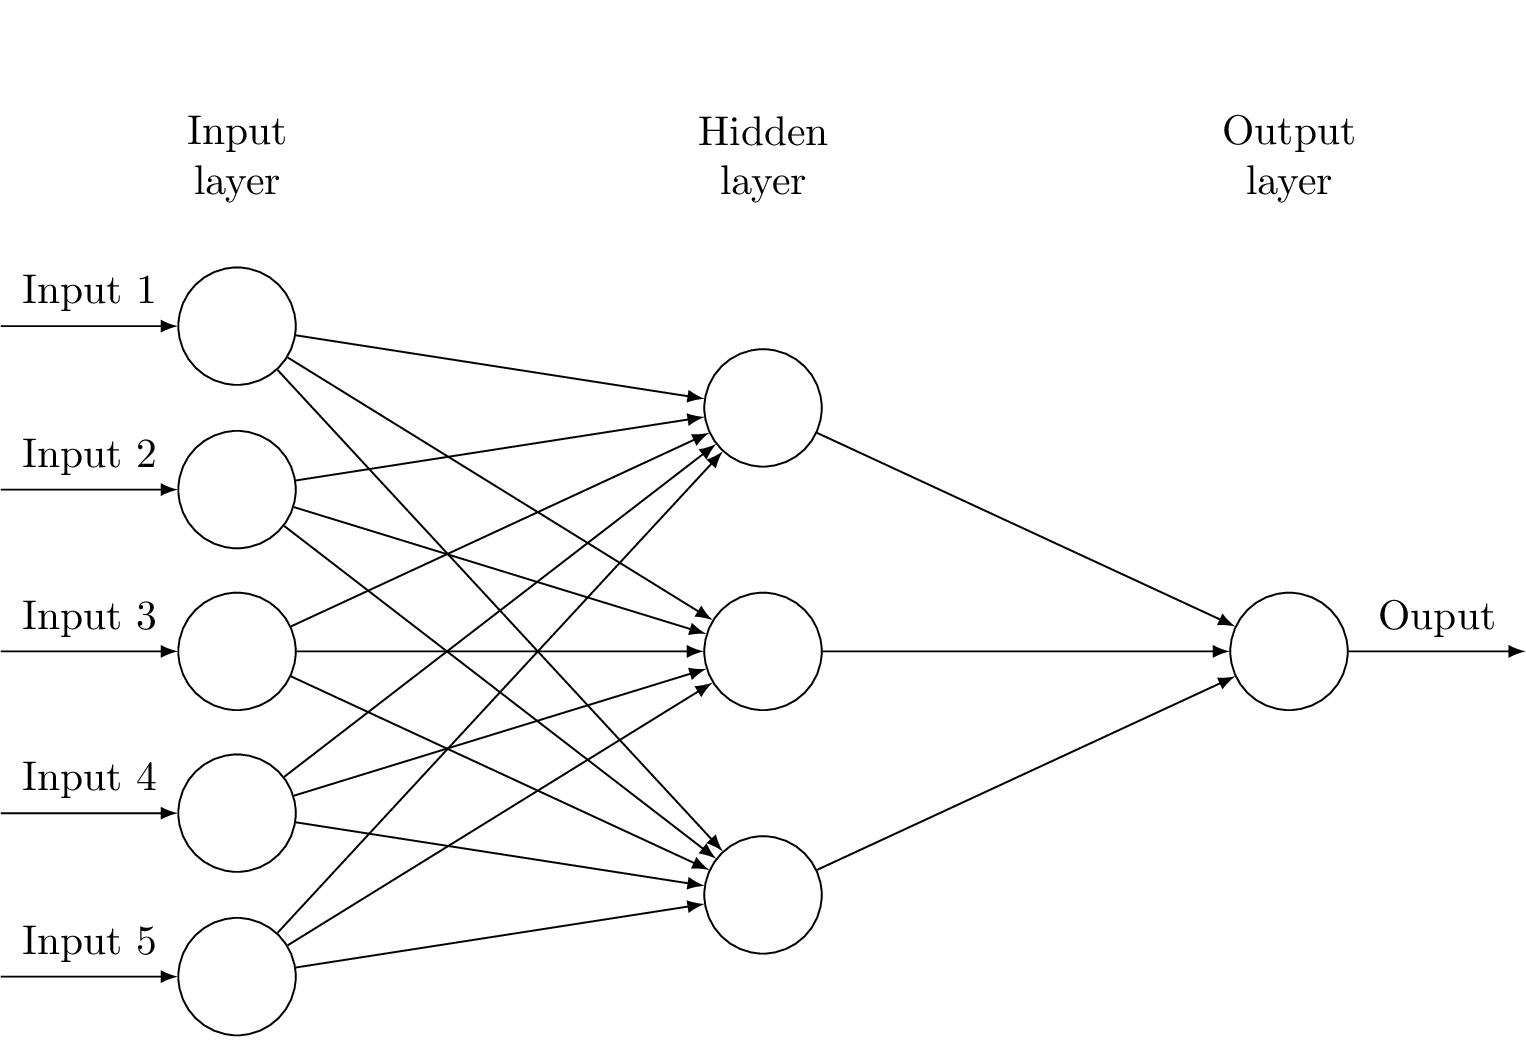
\includegraphics[width=0.8\textwidth]{../assets/mlp_model.png}
    \end{figure}
\end{frame}

\begin{frame}{Scetch of the algorithm}
    TODO
\end{frame}

\printbibliography

\end{document}